\begin{center}
    \begin{minipage}{0.45\textwidth}
        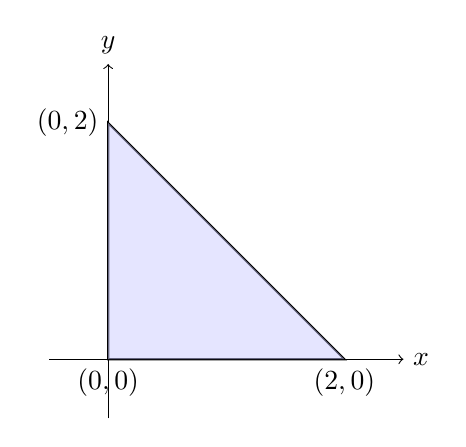
\begin{tikzpicture}[scale=1.5]
            % Ejes coordenados
            \draw[->] (-0.5,0) -- (2.5,0) node[right] {$x$}; % Dibuja el eje x con una flecha en el extremo derecho
            \draw[->] (0,-0.5) -- (0,2.5) node[above] {$y$}; % Dibuja el eje y con una flecha en el extremo superior

            % Triángulo original en xy
            \draw[thick] (0,0) -- (2,0) -- (0,2) -- cycle; % Dibuja el triángulo con vértices en (0,0), (2,0) y (0,2)

            % Etiquetas de los vértices
            \node[below] at (0,0) {$(0,0)$}; % Etiqueta el vértice (0,0)
            \node[below] at (2,0) {$(2,0)$}; % Etiqueta el vértice (2,0)
            \node[left] at (0,2) {$(0,2)$}; % Etiqueta el vértice (0,2)

            % Área sombreada
            \fill[blue!20,opacity=0.5] (0,0) -- (2,0) -- (0,2) -- cycle; % Rellena el triángulo con un color azul claro y opacidad del 50%
        \end{tikzpicture}
    \end{minipage}
    \hspace{0.0000001\textwidth} % Ajusta este valor para cambiar la separación entre las dos minipages
    \begin{minipage}{0.45\textwidth}
        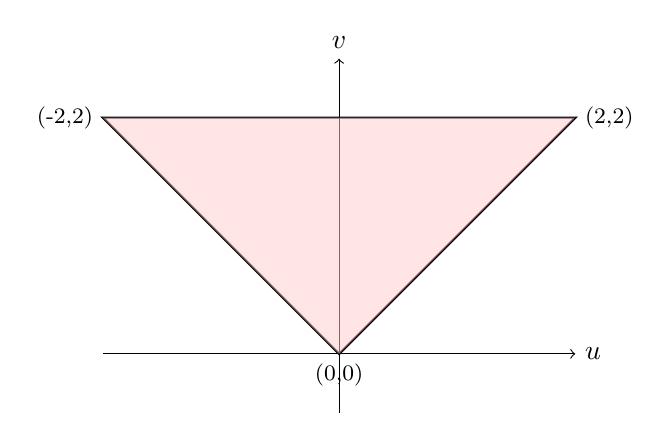
\begin{tikzpicture}[scale=1.5]
            % Ejes coordenados
            \draw[->] (-2,0) -- (2,0) node[right] {$u$};
            \draw[->] (0,-0.5) -- (0,2.5) node[above] {$v$};

            % Triángulo
            \draw[thick] (-2,2) -- (2,2) -- (0,0) -- cycle;

            % Etiquetas de los vértices
            \node[left] at (-2,2) {\footnotesize (-2,2)};
            \node[right] at (2,2) {\footnotesize (2,2)};
            \node[below] at (0,0) {\footnotesize (0,0)};

            \fill[red!20,opacity=0.5] (0,0) -- (2,2) -- (-2,2) -- cycle; % Rellena el triángulo transformado con un color rojo claro y opacidad del 50%
        \end{tikzpicture}
    \end{minipage}
\end{center}
